% !TeX spellcheck = en_US
%% Version 1.2, August 2017
%% This Reference Sheet is free under the terms and conditions of the \LaTeX{} Project Public License Version 1.3c. 
%% Authors: Marion Lammarsch, University of Heidelberg, and Elke Schubert, Stutensee

\documentclass[fontsize=6pt,paper=a4,paper=landscape,twoside=false,parskip=half,
headings=small,numbers=withenddot,usegeometry=true,english]{scrartcl}

\usepackage[utf8]{inputenc}
\usepackage[T1]{fontenc}
\usepackage[ngerman,french,main=english]{babel}
\selectlanguage{english}

\usepackage{cmbright}
\usepackage[scaled=.90]{beramono} 

\usepackage[table]{xcolor}
\usepackage{graphicx}
\arrayrulecolor{gray!60}
\usepackage{geometry}
\geometry{paper=a4paper,landscape, left=6mm,right=6mm, top=8mm,bottom=4mm}
\pagestyle{empty}

\usepackage{tabulary}
\usepackage{multicol}
\usepackage{booktabs}
\usepackage{microtype}
\usepackage{pdfpages}
\usepackage[autostyle=true]{csquotes}	
\usepackage{amsmath,amssymb,nicefrac}
\abovedisplayskip=1pt\belowdisplayskip=0pt\abovedisplayshortskip=0pt\belowdisplayshortskip=0pt
\usepackage{enumitem,pifont,textcomp}
\setlist{noitemsep,itemindent=0pt,leftmargin=1.4em,nosep}
\setlist[itemize]{label*=\ding{223}}
\setlength{\tabcolsep}{2pt}
\usepackage[sticky-per=true,per-mode=fraction]{siunitx}

% Bibliography (here for listings only)
\usepackage[backend=biber,style=verbose]{biblatex}

% Box
\providecommand{\sectionbox}[1]{{\fboxsep0.5em\hspace*{-1.5\fboxsep}%
 \fcolorbox{gray}{gray!3}{%
 \parbox{\columnwidth}{%
 \raggedright #1}}}}

\setlength{\parskip}{1pt}
\renewcommand{\arraystretch}{1.12}

\setkomafont{disposition}{\color{violet}}
\setkomafont{section}{\large}
\setkomafont{subsection}{\normalsize}
\setkomafont{subsubsection}{\normalsize}

\renewcommand*{\thesection}{\Alph{section}}
\RedeclareSectionCommand[beforeskip=-6pt, afterskip=3sp]{section}
\RedeclareSectionCommand[beforeskip=-2pt, afterskip=3sp]{subsection}
\RedeclareSectionCommand[beforeskip=-2pt, afterskip=3sp]{subsubsection}

\renewcommand{\familydefault}{\sfdefault}

% Cprotect ======================
\usepackage{cprotect}
% make boxes robust for verbatim
\let\oldsectionbox\sectionbox
\outer\def\sectionbox{\icprotect\oldsectionbox}

% Hyperref ======================
\usepackage{hyperref}
\renewcommand{\subsectionautorefname}{section}

\definecolor{darkblue}{RGB}{0, 82, 147}		
\hypersetup{
	pdfcreator={LaTeX2e},
	pdfborder=0 0 0,
	breaklinks=true,
	bookmarksopen=true,
	bookmarksnumbered=true,
	linkcolor=darkblue,
	urlcolor=darkblue,
	citecolor=darkblue,
	colorlinks=true,
	pdfauthor=Marion Lammarsch, 
	pdftitle=LaTeX Cheat Sheet,
	pdfcreator=LaTeX2e 
}
\urlstyle{sf}

% Source Code Listings ============
\usepackage{listings}
\definecolor{listinggray}{gray}{0.95}
\lstset{
	backgroundcolor=\color{listinggray},
	basicstyle=\ttfamily\small,
	aboveskip={0.4\baselineskip},
	belowskip={0.4\baselineskip},
	literate={ä}{{\"a}}1 {ö}{{\"o}}1 {ü}{{\"u}}1 {Ä}{{\"A}}1 {Ö}{{\"O}}1 {Ü}{{\"u}}1 {ß}{{\ss}}1 {ô}{{\^o}}1	
}

\lstnewenvironment{mylatex} 
{\lstset{%
	backgroundcolor=\color{listinggray},
	basicstyle=\ttfamily\small,
	tabsize=2,
	language={[LaTeX]TeX},
	%upquote=true,
	aboveskip={0.4\baselineskip},
	belowskip={0.4\baselineskip},
	abovecaptionskip={\baselineskip},
	belowcaptionskip={0\baselineskip},
	columns=fixed,
	showstringspaces=false,
	extendedchars=true,
	linewidth=.96\linewidth,
	xleftmargin=.04\linewidth,
	frameround=fttt,
	framexleftmargin={2pt},
	framexrightmargin={2pt},
	prebreak = \raisebox{0ex}[0ex][0ex]{\ensuremath{\hookleftarrow}},
	frame=single,
	showtabs=false,
	showspaces=false,
	showstringspaces=false,
	identifierstyle=\ttfamily,
	keywordstyle=\color{darkblue},
	commentstyle=\color[rgb]{0.133,0.545,0.133},
	stringstyle=\color[rgb]{0.8,  0.1,  0.1},
	morekeywords={part,chapter,subsection,subsubsection,paragraph,subparagraph,tableofcontents,%
		listoffigures,listoftables,printacronyms,ihead,ohead,clearscrheadings,clearmainofpairofpagestyles,%
		headmark,pagemark,maketitel,tr,varnothing,renewcommand,usepackage,includegraphics,graphicspath,%
		acsetup,DeclareAcroListStyle,DeclareAcronym,ac,Ac,definecolor,colorlet,textcolor,colorbox,%
		rowcolor,addbibresource,autocite,printbibliography,%	
		nexists,KOMAoptions,PassOptionsToPackage,thesection,thefigure,color,foreignlanguage},
	literate={ä}{{\"a}}1 {ö}{{\"o}}1 {ü}{{\"u}}1 {Ä}{{\"A}}1 {Ö}{{\"O}}1 {Ü}{{\"u}}1 {ß}{{\ss}}1 {ô}{{\^o}}1	
}}{}


\sloppy

% DOCUMENT_BEGIN ===============================================================
\begin{document}

% Split into 4 columns ===========================================================
\begin{multicols}{4}

\parbox{\columnwidth}{
\centering\Large\color{violet}Reference Sheet for a Thesis\\[2pt] with \LaTeX2e{} and \KOMAScript{}
}

\sectionbox{
\begin{itemize}
\item 
All examples were tested with \lstinline+pdflatex+.
\item
The package mentioned in the headings has to be included (see~\ref{sec:pack}).
\item 
Compile three times after last change (esp. docs with references).
\end{itemize}
}


% SECTION ====================================================================================
\section{\LaTeX{} Basics}
% ============================================================================================

\sectionbox{
\subsection{Units}\label{sec:units}
\begin{itemize}
\item
Available units for length and dimensions:\\
\begin{tabular}{@{}*{3}{ll@{\quad}}ll@{}}
\lstinline+bp+ & point (typographic) & \lstinline+mm+ & millimeter & \lstinline+in+ & inch & \lstinline+em+ & width of M \\
\lstinline+px+ & pixel ($\nicefrac{1}{72}$in)     & \lstinline+cm+ & centimeter & \lstinline+pc+ & pica & \lstinline+ex+ & height of x \\
\end{tabular}\\
\item
Document dependent units \textit{z}\lstinline+\textwidth+, \textit{z}\lstinline+\linewidth+, \textit{z}\lstinline+\columnwidth+, \textit{z}\lstinline+\textheight+  with \textit{z} a percentage value, e.g. 
\lstinline+0.55\textwidth+ means 55\% of the actual width of the text.
\item 
\lstinline+\baselineskip+ minimum vertical space between the bottom of two successive lines in a paragraph.
\item
Amounts like \lstinline+\smallskipamount+, \lstinline+\medskipamount+, \lstinline+\bigskipamount+.
\end{itemize}
}

\sectionbox{
\subsection{Reserved Characters (see also \ref{sec:textchars}, cf. \ref{sec:math})}\label{sec:specchars}
\begin{tabular}{@{}lll@{}} \toprule
\texttt{\textbackslash} & introduces a command                    & \lstinline+\textbackslash+\\
\texttt{\{ \}} & embraces arguments, creates logical parts        & \lstinline+\{ \}+\\
\texttt{[ ]}   & embraces \textit{optional} arguments             & \lstinline+[ ]+\\ 
\texttt{\%}    & comments: code after \% will be ignored.         & \lstinline+\%+\\ 
\texttt{\&}    & separates columns in tabular-like environments ~ & \lstinline+\&+\\
\texttt{\#}    & parameter for own command declarations           & \lstinline+\#+\\
\texttt{\$}    & text style math mode (abbr. for \lstinline+\(+\dots\lstinline+\)+)   & \lstinline+\$+\\
\texttt{\textunderscore}\texttt{\textasciicircum} & index/exponent only valid in math mode, e.g. 
$a_{1}^{2}$ & see \ref{sec:textchars}\\
\bottomrule
\end{tabular}\\
}


% SECTION ====================================================================================
\section{Preamble (before \texttt{\textbackslash begin\{document\}})}
% ============================================================================================

\sectionbox{
\subsection{Documentclass (necessary)}\label{sec:options}
Use: \lstinline+\documentclass[+\textit{opt,opt,\dots}\lstinline+]{+\textit{class}\lstinline+}+\\
Recommended classes: \lstinline+scrartcl+, \lstinline+scrreprt+, \lstinline+scrbook+, \lstinline+scrlttr2+\\ Non-\KOMAScript{} classes: \lstinline+beamer+, \lstinline+koma-moderncvclassic+\\[2pt]
\begin{tabular}{@{}ll@{}} \toprule
Common options with default  & Values available (subtotal) \\   \midrule
\lstinline+fontsize=11pt+     & \lstinline+10pt+ | \lstinline+12pt+ (e.g. 12.5pt also valid)\\
\lstinline+paper=a4+, \lstinline+paper=portrait+  & \lstinline+a3+ | \lstinline+a5+ | \lstinline+b4+ | \lstinline+letter+, \lstinline+landscape+ \\
\lstinline+parskip=no+        & \lstinline+half+ | \lstinline+full+\\
\lstinline+headings=big+      & \lstinline+small+ | \lstinline+normal+\\
\lstinline+chapterprefix=false+ & \lstinline+true+\\		
\lstinline+open=right+ (scrbook)& \lstinline+any+ (scrartcl, scrreprt) | \lstinline+left+\\ 
\lstinline+captions=oneline+    & \lstinline+nooneline+\\ 
\lstinline+captions=tablebelow+,\lstinline+figurebelow+ & \lstinline+tableabove+, \lstinline+figureabove+\\ 
\lstinline+toc=nolistof+      & \lstinline+listof+ | \lstinline+listofnumbered+\\
\lstinline+bibliography=totoc+ | \lstinline+totocnumbered+ & \lstinline+nottotoc+ \\
\lstinline+twoside=true+ (scrbook)  & \lstinline+false+ (scrartcl, scrreprt)\\
\lstinline+twocolumn=false+   & \lstinline+true+  \\
\lstinline+draft=false+       & \lstinline+true+ (show overfull boxes)\\   \bottomrule
\end{tabular}
\begin{itemize}
\item
Options of document class are passed to every loaded package.
\item
Set or change options later in file, e.g. \lstinline+\KOMAoptions{twoside=true}+
\end{itemize}
}

\sectionbox{
\subsection{Loading Packages}\label{sec:pack}
\lstinline+\usepackage[+\textit{options}\lstinline+]{+\textit{package}\lstinline+}+\\
\lstinline+\PassOptionsToPackage[+\textit{options}\lstinline+]{+\textit{package}\lstinline+}+
}

\sectionbox{
\subsection{Encoding Settings}
\begin{mylatex}
\usepackage[utf8]{inputenc}   % most IDEs use UTF8
\usepackage[T1]{fontenc}      % most fonts needs T1
\end{mylatex}
}

\sectionbox{
\subsection{Language Settings with \texttt{babel}}
Load: \lstinline+\usepackage[ngerman, main=english]{babel}+ \\
Use: \lstinline+\selectlanguage{+\textit{language}\lstinline+}+ \quad \lstinline+\foreignlanguage{+\textit{language}\lstinline+}{+\textit{text}\lstinline+}+\\
\begin{mylatex}
\documentclass[italian]{scrbook}         % global option
\usepackage[british,main=italian]{babel} % package option
\usepackage{csquotes}    % package csquotes knows italian
\end{mylatex}
}


% SECTION ====================================================================================
\section{Layout}\label{sec:layout}
% ============================================================================================

\sectionbox{
\subsection{Changing Page Layout with \texttt{geometry}}
\begin{itemize}
\item
Let \KOMAScript{} know of \texttt{geometry} by option \lstinline+usegeometry=true+.
\begin{mylatex}
\usepackage[left=2cm, right=2, top=3cm, bottom=4cm,
  bindingoffset=1cm, inlcudeheadfoot]{geometry}
\end{mylatex}
\item 
Auto-completion determines unspecified dimensions (under or over specified as well), here \lstinline+width+ and \lstinline+height+ of text (see~\ref{sec:pagelayout}). 
\item
Other options: \lstinline+paper=a4paper+, \lstinline+landscape|portrait+, \lstinline+includehead+, 
\lstinline+includefoot+, \lstinline+includeheadfoot+, \lstinline+twocolumn+
\item
Changing page layout mid document: \lstinline+\newgeometry{+ \textit{opt, opt, ...} \lstinline+}+
\end{itemize}
}

\sectionbox{
\subsection{Header and Footer of Page (aka running heading)}
~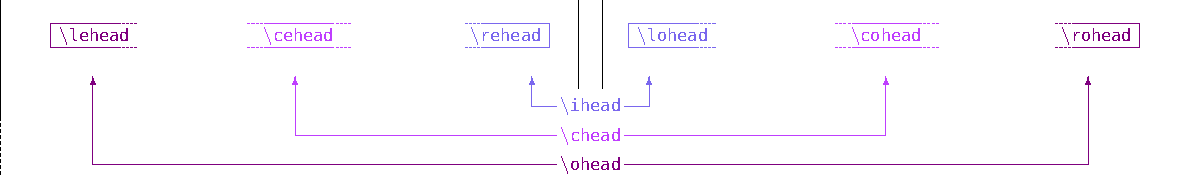
\includegraphics[width=.975\columnwidth]{header-graph.pdf}
\begin{mylatex}
% delete default settings and define your own
\usepackage[automark]{scrlayer-scrpage} 
\clearpairofpagestyles 
\ohead[]{\headmark} \ofoot[\pagemark]{\pagemark}
\end{mylatex}
\begin{mylatex}
% Variant for a thesis with horizontal rules at head and foot
\usepackage[headsepline=0.005pt:,footsepline=0.005pt:, 
plainfootsepline,automark]{scrlayer-scrpage} 
\clearpairofpagestyles
\ohead[]{\headmark} \ofoot[\pagemark]{\pagemark}
\ModifyLayer[addvoffset=-.6ex]{scrheadings.foot.above.line}
\ModifyLayer[addvoffset=-.6ex]{plain.scrheadings.foot.above.line}
\setkomafont{pageheadfoot}{\small}
\end{mylatex}
}

\sectionbox{
\subsection{Linespread with \texttt{setspace}}
Load: \lstinline+\usepackage[onehalfspacing]{setspace}+ for 1.5 line spacing.
}


% SECTION ====================================================================================
\section[Document Structure]{Document Structure (see also \ref{sec:inpfile})}
% ============================================================================================

\sectionbox{
\subsection{Start Document}
\lstinline+\begin{document}+ \textit{Complete document contents.} \lstinline+\end{document}+
}

\sectionbox{
\subsection{Title}
simple title: \lstinline+\author{+\textit{text}\lstinline+}+~ \lstinline+\title{+\textit{text}\lstinline+}+~ \lstinline+\date{\today}+~ \lstinline+\maketitle+\\
title page self designed: \lstinline+\begin{titlepage}+ \textit{text} \lstinline+\end{titlepage}+
}

\sectionbox{
\subsection{Table of Contents, List of Figures (for other List of see \ref{sec:acro} \& \ref{sec:bibl})}
\lstinline+\tableofcontents+ \qquad \lstinline+\listoftables+ \qquad \lstinline+\listoffigures+\\
KOMAoption \lstinline+toc=listof+ (see~\ref{sec:options}) generates entries for TOC.
}

\sectionbox{
\subsection{Headings}
\begin{tabular}{@{}l@{\qquad}l@{\qquad}l@{}}  \toprule
\lstinline+\part{+\textit{title}\lstinline+}+    
  & \lstinline+\chapter{+\textit{title}\lstinline+}+ \\  
\lstinline+\section{+\textit{title}\lstinline+}+   
  & \lstinline+\subsection{+\textit{title}\lstinline+}+  
  & \lstinline+\subsubsection{+\textit{title}\lstinline+}+ \\
\lstinline+\paragraph{+\textit{title}\lstinline+}+ 
  & \lstinline+\subparagraph{+\textit{title}\lstinline+}+  \\ \bottomrule
\end{tabular}
\begin{itemize}
\item 
\lstinline+\chapter+ only valid in documentclass \lstinline+scrbook+ and \lstinline+scrreprt+\\ 
\item 
Use \lstinline+*+ variants for headings without numbering, no change in counter and no entry in table of contents.
\item 
Use the optional parameter for short titles in headings and table of contents, e.g. 
\lstinline+\section[+\textit{short title}\lstinline+]{+\textit{title}\lstinline+}+
\item 
Use \lstinline+\addpart+, \lstinline+\addchap+ or \lstinline+\addsec+ for unnumbered headings, but with  
running heading and entry in table of contents.\\
The \lstinline+*+ variants delete the running heading. 
\item
Layout of paragraph and subpargraph similar to other headings:\\
\lstinline+\RedeclareSectionCommands[afterskip=1sp]{paragraph,subparagraph}+\\ 
\lstinline+\setcounter{secnumdepth}{\subparagraphnumdepth}+\\
\lstinline+\setcounter{tocdepth}{\subparagraphtocdepth}+ 
\end{itemize}}

\sectionbox{
\subsection[Justification]{Justification\phantom{g}}
\begin{tabular}{@{}l@{\qquad}l@{\qquad}l@{}} 		\toprule
	Environment                    & Declaration               & Other \\ \midrule
	\lstinline+\begin{center}+     & \lstinline+\centering+    & \textit{text} \lstinline+\par\vfill+ \textit{text}\\
	\lstinline+\begin{flushleft}+  & \lstinline+\raggedright+  & \textit{text} \lstinline+\hfill+ \textit{text}\\
	\lstinline+\begin{flushright}+ & \lstinline+\raggedleft+   & \lstinline+\raggedbottom+, \lstinline+\flushbottom+\\ 			\bottomrule
\end{tabular}
%For longer text use package \texttt{ragged2e}.
}

\sectionbox{
\subsection{Lists}
\begin{tabular}{@{}ll}
\lstinline+\begin{itemize}+ with bullets        & \lstinline+\item+ or \lstinline+\item[+\textit{symbol}\lstinline+]+\\
\lstinline+\begin{enumerate}+ with numbers      & \lstinline+\item+\\
\lstinline+\begin{description}+ with bold words & \lstinline+\item[+\textit{word}\lstinline+]+\\
\lstinline+\begin{labeling}[+\textit{separator}\lstinline+]{+\textit{labelinglabel}\lstinline+}+ &
\lstinline+\item[+\textit{word}\lstinline+]+
\end{tabular}
\begin{mylatex}
\begin{enumerate}
  \item First item
  \item Second item\label{it:second} % see References
\end{enumerate}
\end{mylatex}
}

\sectionbox{
\subsection{Enhanced Lists with \texttt{enumitem}}
Load: \lstinline+\usepackage{enumitem}+\\[1pt]
\begin{minipage}[t]{.65\columnwidth}
Example (for enumerate):\\
\lstinline+\setlist[enumerate,1]{label=\Alph*)}+\\
\lstinline+\setlist[enumerate,2]{label=\alph*)}+\\
\lstinline+\setlist[enumerate,3]{label=\roman*)}+\\
\lstinline+\setlist[enumerate,4]{label=\arabic*)}+\\
\end{minipage}\hfill
\begin{minipage}[t]{.33\columnwidth}
\setlist[enumerate,1]{label=\Alph*)}
\setlist[enumerate,2]{label=\alph*)}
\setlist[enumerate,3]{label=\roman*)}
\setlist[enumerate,4]{label=\arabic*)}
\setlist[enumerate]{nosep}
\vspace*{2pt}
\begin{enumerate}
\item one 
\begin{enumerate}
	\item one 
	\item two
\end{enumerate}
\item two
\end{enumerate}%
\end{minipage}\\[-2pt]
\begin{minipage}[t]{.65\columnwidth}
Example (for legal list):\\ 
\lstinline+\newlist{legal}{enumerate}{10}+\\
\lstinline+\setlist[legal]{label*=\arabic*.,noitemsep}+\\ 
Use: \lstinline+\begin{legal}+ \lstinline+\item ...+\lstinline+\end{legal}+
\end{minipage}\hfill
\begin{minipage}[t]{.3\columnwidth}
\newlist{legal}{enumerate}{10} 
\setlist[legal]{label*=\arabic*.,noitemsep,nosep} 
\begin{legal}
 \item one
 \begin{legal}
  \item two 
  \begin{legal}
   \item three 
   \item strawberry
  \end{legal}			
 \end{legal}	
\end{legal}%
\end{minipage}%
}

\sectionbox{
\subsection{Separate Files}
\begin{itemize}
\item 
After preamble within the text place:\lstinline+\include{+\textit{file}\lstinline+}+
Text starts and ends on a new page.
\textit{file} has to be in the same directory as the master file. 
Otherwise specify a path: \lstinline+\include{+\textit{path}\lstinline+/+\textit{file}\lstinline+}+
\item 
In preamble place: \lstinline+\includeonly{+\textit{file1},\textit{file2}\lstinline+}+ to run only these files.
\item 
Use \lstinline+\input{+\textit{file}\lstinline+}+ includes a file without starting/ending on a new page (\lstinline+\includeonly+ not valid).
\end{itemize}
}


% SECTION ====================================================================================
\section{Text}
% ============================================================================================
\sectionbox{
\subsection{Paragraphs ($\approx$ ``new idea in content'')}\label{sec:para}
Paragraphs are separated by an empty line in the code or by \lstinline+\par+.\\
A \lstinline+\\+ produces a new line -- use sparingly, seldom needed outside tabulars.\\
Correct Overfull Box Warnings with more than 4pt (look into log file).
}

\sectionbox{
\subsection{Text Symbols/Characters (see also \ref{sec:specchars})}\label{sec:textchars}
A lot of diacritic symbols can be typed directly, e.g. è é ê ñ ç \\
\begin{tabular}{*{6}{l}}\toprule
\S              &  \lstinline+\S+          &
\textunderscore & \lstinline+\textunderscore{}+    &
\textasciitilde &  \lstinline+\textasciitilde{}+ \\
\textasciicircum & \lstinline+\textasciicircum{}+ &
\ldots          &  \lstinline+\ldots+      &
\textbar        &  \lstinline+\textbar+    \\
\bottomrule
\end{tabular}\\
Other symbols need packages, e.g. \texteuro ~ \lstinline+\texteuro+ (\lstinline+textcomp+)\\ 
}

\sectionbox{
\subsection[Fonts]{Fonts\phantom{g}}
\begin{tabular*}{\columnwidth}{@{}l@{\extracolsep\fill}ll@{}} \toprule
Command      &    Declaration &   Effect \\ \midrule
\lstinline+\textrm{+\textit{text}\lstinline+}+                    & %
\lstinline+{\rmfamily +\textit{text}\lstinline+}+               & %
\textrm{Roman family} \\
\lstinline+\textsf{+\textit{text}\lstinline+}+                    & %
\lstinline+{\sffamily +\textit{text}\lstinline+}+               & %
\textsf{Sans serif family} \\
\lstinline+\texttt{+\textit{text}\lstinline+}+                    & %
\lstinline+{\ttfamily +\textit{text}\lstinline+}+               & %
\texttt{Typewriter family} \\
\lstinline+\textmd{+\textit{text}\lstinline+}+                    & %
\lstinline+{\mdseries +\textit{text}\lstinline+}+               & %
\textmd{Medium series} \\
\lstinline+\textbf{+\textit{text}\lstinline+}+                    & %
\lstinline+{\bfseries +\textit{text}\lstinline+}+               & %
\textbf{Bold series} \\
\lstinline+\textup{+\textit{text}\lstinline+}+                    & %
\lstinline+{\upshape +\textit{text}\lstinline+}+                & %
\textup{Upright shape} \\
\lstinline+\textit{+\textit{text}\lstinline+}+                    & %
\lstinline+{\itshape +\textit{text}\lstinline+}+                & %
\textit{Italic shape} \\
\lstinline+\textsl{+\textit{text}\lstinline+}+                    & %
\lstinline+{\slshape +\textit{text}\lstinline+}+                & %
{\usefont{T1}{cmr}{m}{sl}Slanted shape} \\
\lstinline+\textsc{+\textit{text}\lstinline+}+                    & %
\lstinline+{\scshape +\textit{text}\lstinline+}+                &  %
% textsc from computer modern because cmbright does not have scshape
{\usefont{T1}{cmr}{m}{sc}Small Caps shape} \\
\multicolumn{3}{l}{More general commands:}\\
\lstinline+\emph{+\textit{text}\lstinline+}+                      & %
\lstinline+{\em +\textit{text}\lstinline+}+                     & %
\emph{Emphasized} \\
\lstinline+\textnormal{+\textit{text}\lstinline+}+                & %
\lstinline+{\normalfont +\textit{text}\lstinline+}+             & %
\textnormal{Document font} \\							\bottomrule
\end{tabular*}\\
Example: \lstinline+\setkomafont{section}{\scshape}+
%%The commands produce better results, e.g.  t\textsl{tt}t (textsl) than the declarations, e.g. t{\slshape tt}t (slshape)!
}

\sectionbox{
\subsection{Font Size}
Font size is relative to the base font size, specified in the document class.\\
\renewcommand{\arraystretch}{0.9}
\begin{tabular}{@{}ll@{}}
\lstinline+\tiny+                  &  \tiny{tiny} \\
\lstinline+\scriptsize+            &  \scriptsize{scriptsize} \\
\lstinline+\footnotesize+          &  \footnotesize{footnotesize} \\
\lstinline+\small+                 &  \small{small} \\
\lstinline+\normalsize+            &  \normalsize{normalsize} \\
\lstinline+\large+                 &  \large{large}
\end{tabular} \qquad~~~	
\begin{tabular}{@{}ll@{}}	
\lstinline+\Large+                 &  \large{Large} \\[2pt]  
\lstinline+\LARGE+                 &  \Large{LARGE} \\[2pt]
\lstinline+\huge+                  &  \LARGE{huge} \\[2pt]
\lstinline+\Huge+                  &  \huge{Huge}	\\[2pt]	
\end{tabular}\\
Use: \lstinline+{\small+ \textit{text}\lstinline+}+ or \lstinline+{\huge+ \textit{text}\lstinline+\par}+ to limit the size change.\\
Example: \lstinline+\setkomafont{pageheadfoot}{\small}+
}

\sectionbox{
\subsection{Colors with \texttt{xcolor}}
\begin{mylatex}
\usepackage{xcolor}	
\definecolor{DarkBlue}{RGB}{0, 115, 207}
\colorlet{col_section}{DarkBlue}
\textcolor{red}{text in red} or {\color{red}text}
\colorbox{gray!25}{color gray faded by 25\%}
\end{mylatex}
Predefined colors:\\ 
\texttt{\colorbox{gray!25}{\textcolor{white}{white}} \textcolor{gray}{gray} black \textcolor{red}{red} \textcolor{green}{green} \textcolor{blue}{blue} \textcolor{cyan}{cyan} \textcolor{magenta}{magenta} \textcolor{yellow}{yellow}}\\
Fade a color with \textit{color}\lstinline+!+\textit{value} between 0 and 100\\
Headings in color: \lstinline+\setkomafont{disposition}{\color{+\textit{color}\lstinline+}}+
}

\sectionbox{
\subsection[Footnotes]{Footnotes\phantom{g}}
\begin{tabular}{@{}p{.32\columnwidth}p{.65\columnwidth}@{}}\toprule
\lstinline+\footnote{+\textit{text}\lstinline+}+  &  Print footnote marker in text and footnote at bottom of page \\
\lstinline+\footnotemark+  &  Print footnote marker in text (e.g. within tabular or caption)\\
\lstinline+\footnotetext{+\textit{text}\lstinline+}+  &  Print footnote at bottom of page \\
\bottomrule\end{tabular}\\
}

\sectionbox{
\subsection{References with \texttt{hyperref} (loads \texttt{url} implicitly)}
\begin{tabular}{@{}p{.30\columnwidth}p{.69\columnwidth}@{}}\toprule
\lstinline+\autocite{+\textit{citekey}\lstinline+}+ & Cite a bibliographic reference (package \texttt{biblatex})\\
\lstinline+\label{+\textit{marker}\lstinline+}+   &  Set a marker for cross reference, 
often if the form \lstinline+\label{sec:item}+ or \lstinline+\label{fig:diag1}+ \\
\end{tabular}\\
\begin{tabular}{@{}p{.42\columnwidth}p{.55\columnwidth}@{}}
\lstinline+\autoref{+\textit{marker}\lstinline+}+ &  Give type name and number of marker \\
\lstinline+\autopageref{+\textit{marker}\lstinline+}+ &  Give abbreviation of ``page'' and page number of marker \\
\lstinline+\url{+\textit{url}\lstinline+}+ & Print clickable web page\\
\lstinline+\href[+\textit{options}\lstinline+]{+\textit{url}\lstinline+}{+\textit{text}\lstinline+}+
& Print clickable link\\
\lstinline+\hyperref[+\textit{marker}\lstinline+]{+\textit{text}\lstinline+}+
& Print clickable reference\\
\bottomrule\end{tabular}\\
Style: \lstinline+\urlstyle{+\textit{xx}\lstinline+}+ with \textit{xx} a style like ``tt'', ``rm'', ``sf'' or ``same''. \\
Names for autoref  (package \texttt{babel}):\\ ~~\lstinline+\renewcaptionname{+\textit{language}\lstinline+}{\+\textit{typename}\lstinline+autorefname}{+\textit{text}\lstinline+}+,\\ 
~~e.g. \lstinline+\renewcaptionname{english}{\subsectionautorefname}{section}+%
}

\sectionbox{
\subsection{Acronyms with \texttt{acro}}\label{sec:acro}
\begin{mylatex}
\usepackage{acro,hyperref,longtable,tabu} %next 5 to praeambel
\acsetup{list-style=longtabu,list-heading=addchap}
\DeclareAcroListStyle{longtabu}{table}{table=longtabu,
  table-spec=@{}>{\bfseries}lX@{}}
\DeclareAcronym{ecm}{short=EM,long=Electro Machining}
...
\ac{EM} or \Ac{EM} for capitalized first letter
\printacronyms
\end{mylatex}
}


% SECTION ====================================================================================
\section{Figures \& Tables (floating environments)}
% ============================================================================================

\sectionbox{
\subsection{Figures with \texttt{graphicx}}\label{sec:figure}
Load: \lstinline+\usepackage{graphicx}+\\
Use: \lstinline+\includegraphics[+\textit{opt}\lstinline+]{+\textit{file}\lstinline+}+ (png, jpg, pdf)\\[2pt]
With `figure' the environment to place a graphic is meant. The figure caption is printed where the caption command is placed in the input.  Extra vertical space is controlled by the KOMAoption \lstinline+captions+ (see~\ref{sec:options}).\\
Use: \lstinline+\begin{figure}[+\textit{pos}\lstinline+] ..\caption{..}\label{fig:x}+ \lstinline+\end{figure}+\\
Parameter: \textit{pos} is a suggestion for placing, it can be ignored by \TeX{}. Possible values are combinations of \lstinline+t+ (top), \lstinline+h+ (here), \lstinline+b+ (bottom), \lstinline+!+ (try  harder), \lstinline+p+ (separate page).\\
Hint: Define a path to the graphic files (no blanks in folder names; no special characters in file names)
\lstinline+\graphicspath{ {+\textit{folder}\lstinline+/}{+\textit{folder}\lstinline+/}+\dots\lstinline+ }+
\begin{mylatex}
\graphicspath{ {img/} } %subfolder for images; set in preambel
\begin{figure}\centering
 \includegraphics[width=.8\columnwidth]{pic.jpg}
 \caption[Short title]{Long title}\label{fig:ff}
\end{figure}
\end{mylatex}
\begin{itemize}
\item 
Numbering throughout the whole document (scrbook) with package \lstinline+chngcntr+:
\lstinline+\counterwithout{figure}{chapter}+ (same for table)
\item 
Figure name:
\lstinline+\renewcaptionname{+\textit{language}\lstinline+}{\figurename}{+\textit{text}\lstinline+}+\\
\lstinline+\renewcaptionname{+\textit{language}\lstinline+}{\figureautorefname}{+\textit{text}\lstinline+}+
\end{itemize}
}\\[6pt]
\parbox{1.005\columnwidth}{\hfill\small typesetted with cmbright, \today}

\sectionbox{
\subsection{Subfigures with \texttt{subcaption}}
Load: \lstinline+\usepackage{subcaption}+\\
Use: \lstinline+\begin{subfigure}[+\textit{pos}\lstinline+]{+\textit{width}\lstinline+}+ \dots{} \lstinline+\end{subfigure}+ 
\begin{mylatex}
\begin{figure}[ht] \centering
 \begin{subfigure}[t]{0.5\textwidth}
  \centering \includegraphics[height=1.2in]{figure-a}
  \caption{Subcaption 1}\label{fig:SubFig1}\end{subfigure}
 \begin{subfigure}[t]{0.5\textwidth}
  \centering \includegraphics[height=1.2in]{figure-b}
  \caption{Subcaption 2}\label{fig:SubFig2}\end{subfigure}
 \caption{Caption of complete figure}\label{fig:Fig1}
\end{figure}
\end{mylatex}
}

\sectionbox{
\subsection{Tables width aligned material}
With `table' the environment to place aligned material is meant. The table caption is printed where the caption command is placed in the input.  For positioning options see~\ref{sec:figure}.
\begin{mylatex}
\KOMAoptions{captions=tableabove} % move to praeambel
\begin{table}[htbp] \centering
 \caption{Table caption}\label{tab:exp}
 \begin{tabular}{@{}ll@{}} 
  \emph{Name} & \emph{Desc.}\\ \hline
  tikz2pdf    & Python script\\
  LaTable     & visual table editor
 \end{tabular}
\end{table}
\end{mylatex}
Use: \lstinline+\begin{tabular}[c b t]{@{} l r c | p{+\textit{unit}\lstinline+}}+\\
Column separation: \lstinline+@{\hspace{+\textit{unit}\lstinline+}}+ or \lstinline+\setlength{\tabcolsep}{+\textit{unit}\lstinline+}+\\
Row separation: \lstinline+\\[+\textit{unit}\lstinline+]+ or \lstinline+\renewcommand{\arraystretch}{+\textit{unit}\lstinline+}+\\		
Partial lines: \lstinline+\cline{2-3}+ instead of \lstinline+\hline+\\
Additional packages: \texttt{array}, \texttt{longtable}, \texttt{booktabs}, \texttt{tabu},\\ 
~~\texttt{xcolor} with option \lstinline+table+, \texttt{tabularx}, \texttt{tabulary}
}

\sectionbox{
\subsection{Colored Table}
\begin{mylatex}
\usepackage[table]{xcolor} % move to praeambel
\rowcolors{1}{}{lightblue} % {start row}{odd-row}{even-row}
\begin{tabular}{clr} ... \end{tabular}
\end{mylatex}
}

\sectionbox{
\subsection{Suppress Floating with \texttt{float}}
For a thesis most students want to control the placing of figures and tables themselves.
One way is more control with \texttt{placeins}.
Another way is to avoid the environments figure and table using \lstinline+\captionof+. 
Quick and dirty is an additional positioning parameter using \texttt{float}:\\
Load: \lstinline+\usepackage{float,scrhack}+\\
Use: \lstinline+\begin{figure}[H]+, \lstinline+\begin{table}[H]+ 
}

\sectionbox{
\subsection{Source Code Listings with \texttt{listings}}
Load: \lstinline+\usepackage{listings}+\\
Options: \lstinline+\lstset{ basicstyle=\ttfamily\small, language=Python,+\\
~~\lstinline+numbers=left, keywordstyle=\color{blue}\bfseries }+\\
~~See option \lstinline+literate+ for Umlauts (\lstinline+literate={+{\small\texttt{ä}}\lstinline+}{{\"a}}1)+\\
Languages: C, C++, Java, Matlab, Python, HTML, XML, \dots\\
\begin{tabular}{@{}ll@{}}
Use: & Environment: \lstinline+\begin{lstlisting}+ \textit{code} \lstinline+\end{lstlisting}+\\
     & In line: \lstinline:\lstinline+:\textit{code}\lstinline:+: (same start- and end char)\\
     & File: \lstinline+\lstinputlisting{+\textit{filename}\lstinline+}+
\end{tabular}
\lstset{language=Python,
	basicstyle=\ttfamily\tiny,
	extendedchars=false,
	numbers=left,
	numbersep=12pt,
	keywordstyle=\color{blue}\bfseries,
	commentstyle=\color{gray!80},
	stringstyle=\color{cyan!40},
	showstringspaces=false,
	linewidth=.96\linewidth,
	xleftmargin=.12\linewidth,
	frameround=fttt,
	framexleftmargin={2pt},
	framexrightmargin={2pt}
}
\begin{lstlisting}
# Python selection
secret=42
guess=int(input("Enter number: "))
if guess==secret: 
    print ("You won!")
elif guess<secret:
    print ("No, secret number bigger.")
else:
    print ("No, secret number is smaller.") 
\end{lstlisting}
}

\sectionbox{
\subsection{Boxes and Rules}\label{sec:boxrule}
Normal: \lstinline+\parbox[pos][height][contentpos]{width}{text}+ or\\
\lstinline+\begin{minipage}[pos][height][contentpos]{width}text+\lstinline+\end{minipage}+\\
Lift Text: \lstinline+\raisebox{lift}[height][depth]{text}+\\
Framed Box: \lstinline+\fbox{text}+ or \lstinline+\framebox[width][pos]{text}+ \\
Colored Box (\texttt{xcolor}): \lstinline+\colorbox{backgroundcolor}{text}+\\ 
Framed colored Box: \lstinline+\fcolorbox{bordercolor}{backgroundcolor}{text}+\\
Resize (\texttt{graphicx}): \lstinline+\scalebox{10}{Giant}+\\
Lengths: \lstinline+\setlength{\fboxsep}{+\textit{unit}\lstinline+}+, \lstinline+\setlength{\fboxrule}{+\textit{unit}\lstinline+}+
}


% SECTION ====================================================================================
\section{Bibliography with \texttt{biblatex} \& External Processor \texttt{biber}}\label{sec:bibl}
% ============================================================================================

\sectionbox{
\subsection{Entry types}
\begin{tabular}{@{}ll@{\qquad}ll@{}}
\lstinline+@article+         &  \lstinline+@book+            &  \lstinline+@inbook+     \\
\lstinline+@collection+      &  \lstinline+@incollection+    &  \lstinline+@manual+     \\
\lstinline+@misc+            &  \lstinline+@online+          &  \lstinline+@patent+     \\ 
\lstinline+@phdthesis+       &  \lstinline+@proceedings+     &  \lstinline+@periodical+ \\
\lstinline+@report+          &  \lstinline+@techreport+      &  \lstinline+@thesis+     \\
\end{tabular}
}

\sectionbox{
\subsection{Entry Fields (example see~\ref{sec:inpfile})}
\begin{tabular}{@{}lllll@{}}
\lstinline+author+ & \lstinline+title+& \lstinline+journal+& \lstinline+year+& \lstinline+volume+\\
\lstinline+editor+ & \lstinline+publisher+& \lstinline+institution+& \lstinline+school+& \lstinline+series+\\
\lstinline+pages+ & \lstinline+organization+& \lstinline+number+& \lstinline+note+& \lstinline+key+
\end{tabular}
}

\sectionbox{
\subsection{Styles}
\begin{tabular}{@{}llllll@{}}
\lstinline+alphabetic+ & \lstinline+authoryear+ & \lstinline+authortitle+ &\lstinline+numeric+ & \lstinline+mla+ & \lstinline+verbose+\\ 
\lstinline+chem-acs+   & \lstinline+phys+ & \lstinline+nature+ & \lstinline+science+ & \lstinline+ieee+& \lstinline+apa+\\
\end{tabular}\\
See \url{https://de.sharelatex.com/learn/Biblatex_bibliography_styles}
}

\sectionbox{
\subsection{Example}
\begin{mylatex}
% in preambel
\usepackage[autostyle=true]{csquotes} % Load
\usepackage[backend=biber,style=nature,language=british]
  {biblatex} % Load
\addbibresource{mybibliographyfile.bib} % Define
% anywhere within the document
\autocite{citekey} % Use
\printbibliography % Print
\end{mylatex}	
KOMAoption \lstinline+bibliography+ (see~\ref{sec:options}) generates entry for TOC.
}

\sectionbox{
\subsection{External Processor}
IDEs like \TeX{}studio include the external processor, select \texttt{biber} as bibliography tool for `build' in preferences, otherwise run \texttt{biber} explicitly.%
}


% SECTION ====================================================================================
\section{Math}\label{sec:math}
% ============================================================================================
\sectionbox{
\subsection{Math mode (Standard \LaTeX{})}
Textstyle: \lstinline:\(x^2 + 4\): $\leadsto$ \(x^2 + 4\) as part of the text.\\
Displaystyle: \lstinline:\[ x^2 + 4 \]: $\leadsto$ separat line, centered\\
Equation: \lstinline+\begin{equation}+ \dots{} \lstinline+\end{equation}\label{+\textit{name}\lstinline+}+ 
\begin{equation}
\lambda := \lim\limits_{x_1 \rightarrow \infty}    \int\limits_{x_0}^{x_1} \frac{ f\left(\frac{t}{2}\right) }{ \sqrt[n]{t^2 + \sin^2(t) } } \; \mathrm{d}t \stackrel{!}\le 1
\end{equation}
\begin{itemize}
\item Use \lstinline+*+ variant for unnumbered equation (without label).
\item Package option for equation position: \lstinline+fleqn+  fixed indent from the left margin instead of centered.
\item Options for positions of equation number: \lstinline+leqno+ or \lstinline+reqno+. 
\end{itemize}
}

\sectionbox{
\subsection{Important Symbols in Math}\label{mathsymbols}
{\setlength{\tabcolsep}{4pt}
\begin{tabular}{@{}cl@{\hspace{2em}}cl@{\hspace{2em}}cl@{\hspace{2em}}cl}\toprule
$+$    & \lstinline+++    & $-$       & \lstinline+-+       & $\pm$     & \lstinline+\pm+     & $\mp$         & \lstinline+\mp+        \\
$<$    & \lstinline+<+    & $\le$     & \lstinline+\le+     & $\ll$     & \lstinline+\ll+     & $\cdot$       & \lstinline+\cdot+      \\
$>$    & \lstinline+>+    & $\ge$     & \lstinline+\ge+     & $\gg$     & \lstinline+\gg+     & $\times$      & \lstinline+\times+     \\
$=$    & \lstinline+=+    & $\ne$     & \lstinline+\ne+     & $\equiv$  & \lstinline+\equiv+  & $\approx$     & \lstinline+\approx+    \\
$|$    & \lstinline+|+    & $\perp$   & \lstinline+\perp+   & $\mid$    & \lstinline+\mid+    & $\parallel$   & \lstinline+\parallel+  \\
$f'$   & \lstinline+f'+   & $\nabla$  & \lstinline+\nabla+  & $\Delta$  & \lstinline+\Delta+  & $\partial$    & \lstinline+\partial+   \\
$\in$  & \lstinline+\in+  & $\forall$ & \lstinline+\forall+ & $\exists$ & \lstinline+\exists+ & $\nexists$    & \lstinline+\nexists+   \\
$\cap$ & \lstinline+\cap+ & $\cup$    & \lstinline+\cup+    & $\notin$  & \lstinline+\notin+  & $\setminus$   & \lstinline+\setminus+  \\
$\ell$ & \lstinline+\ell+ & $\angle$  & \lstinline+\angle+  & $\circ$   & \lstinline+\circ+   & $\emptyset$   & \lstinline+\emptyset+  \\
$\lor$ & \lstinline+\lor+ & $\land$   & \lstinline+\land+   & $\lnot$   & \lstinline+\lnot+   & $\varnothing$ & \lstinline+\varnothing+\\
$\top$ & \lstinline+\top+ & $\bot$    & \lstinline+\bot+    & $\infty$  & \lstinline+\infty+  & $\propto$     & \lstinline+\propto+    \\
\bottomrule\end{tabular}}
}

\sectionbox{
\subsection{Math Functions (upright typeface)}
\begin{tabular}{@{}*{10}{l@{\;}}l@{}} \toprule
\lstinline+\arccos+&\lstinline+\arcsin+&\lstinline+\arctan+&\lstinline+\arg+&\lstinline+\cos+&\lstinline+\cosh+&\lstinline+\cot+&\lstinline+\coth+&\lstinline+\csc+&\lstinline+\deg+&\lstinline+\det+\\
\lstinline+\dim+&\lstinline+\exp+&\lstinline+\gcd+&\lstinline+\hom+&\lstinline+\inf+&\lstinline+\ker+&\lstinline+\lg+&\lstinline+\lim+&\lstinline+\liminf+&\multicolumn{2}{@{\;}l}{$\backslash$\texttt{limsup}}\\
\lstinline+\ln+&\lstinline+\log+&\lstinline+\max+&\lstinline+\min+&\lstinline+\Pr+&\lstinline+\sec+&\lstinline+\sin+&\lstinline+\sinh+&\lstinline+\sup+&\lstinline+\tan+&\lstinline+\tanh+\\
\bottomrule
\end{tabular}
For other functions use (package \texttt{amsmath}): \lstinline+\operatorname{+\textit{name}\lstinline+}+, e.g. \lstinline+\operatorname{arcsinh}+ (see also \ref{owncmds}).
}

\sectionbox{
\subsection[More Math Functions]{More Math Functions\phantom{g}}
{\setlength{\tabcolsep}{6pt}
\begin{tabular}{@{}ll@{\qquad}ll@{\qquad}ll@{\qquad}ll@{}}   \toprule
	$\sum$    & \lstinline+\sum+    & $\prod$   & \lstinline+\prod+   & $\coprod$  & \lstinline+\coprod+\\
	$\int$    & \lstinline+\int+    & $\iint$   & \lstinline+\iint+   & $\iiint$   & \lstinline+\iiint+   & $\oint$   & \lstinline+\oint+\\
	$\vec{a}$ & \lstinline+\vec{a}+ & $\dot{a}$ & \lstinline+\dot{a}+ & $\ddot{a}$ & \lstinline+\ddot{a}+ & $\hat{a}$ & \lstinline+\hat{a}+\\
	\bottomrule
\end{tabular}}
}

\sectionbox{
	\subsection{Fonts and Sizes in Math Mode (some from \AmS{}Math)}
	\lstinline+\mathrm{}+, \lstinline+\mathit{}+, \lstinline+\mathbf{}+, \lstinline+\mathsf{}+, \lstinline+\mathtt{}+, \lstinline+\boldmath{}+\\
	\lstinline+\mathbb{}+ e.g. $\mathbb{AZ}$, \lstinline+\mathcal{}+ e.g. $\mathcal{AZ}$, \lstinline+\mathfrak{}+ e.g. $\mathfrak{AZ}$\\
	\lstinline+\displaystyle+, \lstinline+\scriptstyle+, \lstinline+\scriptscriptstyle+, \lstinline+\textstyle+\\
	\lstinline+\boldsymbol{}+ 
}

\sectionbox{
\subsection{Often used Math Expressions}
\renewcommand{\arraystretch}{1.5}
\everymath{\displaystyle}
\begin{tabular}{@{}ll@{\qquad\quad}ll@{}}
$x^{n+1}$ & \lstinline:x^{n+1}: & $E_{\mathrm{kin}}$ & \lstinline+E_{\mathrm{kin}}+ \\
$\frac{a+b}{2}$ & \lstinline:\frac{a+b}{2}: & $\sqrt[n]{a^2+b^2}$ & \lstinline:\sqrt[n]{a^2+b^2}:\\
$x_1 , \ldots, x_n$~  & \lstinline+x_1, \ldots, x_n+ & $x_1 + \cdots + x_n$~ & \lstinline:x_1 + \cdots + x_n: \\	
\end{tabular}\\[6pt]
\newcommand{\myvec}[1]{\ensuremath{\underline{\boldsymbol {#1}}}}
\begin{tabular}{@{}lm{.8\columnwidth}@{}}
$\left( a + \frac12 \right)^2$ & \lstinline:\left( a + \frac{1}{2} \right)^2:\\[2mm] 
$\sum\limits_{i=1}^{N}$ \quad $\prod\limits_{i=1}^{N}$ & \lstinline+\sum_{i=1}^{N}+ \quad \lstinline+\prod_{i=1}^{N}+\\
$\lim\limits_{a \rightarrow \infty}$ & \lstinline+\lim_{a \rightarrow \infty}+\\ 
$\int\limits_a^b x^2\; \mathrm{d}x$  & \lstinline+\int_a^b x^2\; \mathrm{d}x+\\
$\left. \frac{\mathrm df}{\mathrm{d}x} \right|_{x_0}$ & \lstinline+\left. \frac{\mathrm{d}f}{\mathrm{d}x} \right|_{x_0}+\\
$\myvec{F}_{\perp}$ \quad $\myvec{F}_{\parallel}$ & 
                   \lstinline+\myvec{F}_{\perp}+\footnotemark[1] \quad \lstinline+\myvec{F}_{\parallel}+\footnotemark[1]\\
$\myvec{a}^{\top}$ $A^{\dagger}$ $\boldmath{A}^{*}$  & \lstinline+\myvec{a}^{\top}+\footnotemark[1] \quad \lstinline+A^{\dagger}+ \quad \lstinline+\boldmath{A}^{*}+\\ 
$\stackrel{!}{<}$ \quad $\stackrel{\mathrm{def}}{=}$ & \lstinline+\stackrel{!}{<}+ \quad \lstinline+\stackrel{\mathrm{def}}{=}+\\
$\overset{above}{mid}$ \quad $\underset{below}{mid}$ & \lstinline+\overset{above}{mid}+ \quad \lstinline+\underset{below}{mid}+
\end{tabular} 
$^1$\lstinline+\newcommand{\myvec}[1]{\ensuremath{\underline{\boldsymbol{#1}}}}+%
\everymath{\textstyle}%
}

\sectionbox{
\subsection{Math with \texttt{amsmath} (replacing standard Environments)}
\begin{tabular}{@{}lll@{}}\toprule
\lstinline+equation+ & \lstinline+equation*+ & One line, one equation\\
\lstinline+multline+ & \lstinline+multline*+ & One unaligned multiple-line equation, one number \\
\lstinline+gather+   & \lstinline+gather*+   & Several equations without alignment \\
\lstinline+align+    & \lstinline+align*+    & Several equations with multiple alignments \\
\lstinline+alignat+  & \lstinline+alignat*+  & Multiple alignments, choose spacing between cols\\
\lstinline+flalign+  & \lstinline+flalign*+  & Several equations: horizontally spread form of align \\
\multicolumn{2}{@{}l}{\lstinline+cases+}   & Alignment for cases  \\ 
\multicolumn{2}{@{}l}{\lstinline+split+}   & A simple alignment within a multiple-line equation \\ 
\multicolumn{2}{@{}l}{\lstinline+aligned+} & A ``mini-page'' with multiple alignments \\
\multicolumn{2}{@{}l}{\lstinline+gathered+}& A ``mini-page'' with unaligned equations \\
\bottomrule\end{tabular}
\begin{itemize}
\item 
The content is automatically placed in math mode.
\item
Use \lstinline+\intertext{+\textit{text}\lstinline+}+ to set text within an \texttt{amsmath} environment
\item 
Length parameter to influence vertical spacing within any \texttt{amsmath} environment: \lstinline+\jot+ (e.g. \lstinline+\addtolength{\jot}{1ex}+)
\item
Add singular vertical space for a line via \lstinline+\\[<amount>]+ (see~\ref{sec:units})
\item
Use the \lstinline+spreadlines+ environment from the \texttt{mathtools} package
\item
Length parameters (with standard values) to influence vertical white space around displayed math formulas:
\lstinline+\abovedisplayskip=12pt+,
\lstinline+\belowdisplayskip=12pt+,
\lstinline+\abovedisplayshortskip=0pt+,
\lstinline+\belowdisplayshortskip=7pt+
\end{itemize}
}

\sectionbox{
\subsubsection{\AmS{}Math \texttt{align}}
\vspace*{-4pt}
\begin{minipage}[c]{.52\columnwidth}
\begin{lstlisting}
\begin{align}
y &= d\\
y &= cx+d\nonumber\\ 
y &= bx^{2}+cx+d \label{eq:key}
\end{align}
\end{lstlisting}
\end{minipage}
\begin{minipage}[c]{.45\columnwidth}\setcounter{equation}{0}
{\small
\begin{align}
y &= d\\
y &= cx+d\nonumber\\ 
y &= bx^{2}+cx+d\label{eq:key}
\end{align}}
\end{minipage}

\vspace*{-4pt}
\begin{minipage}[t]{.52\columnwidth}
\begin{lstlisting}
\begin{align*}
y      &= d       & z &= 1\\
y(x)   &= cx+d    & z &= x+1\\
y_{12} &= bx^2+cx & z &= x^2+x+1
\end{align*}
\end{lstlisting}
\end{minipage}
\begin{minipage}[t]{.45\columnwidth}\setcounter{equation}{0}
{\small
\begin{align*}
y      &= d       & z &= 1\\
y(x)   &= cx+d    & z &= x+1\\
y_{12} &= bx^2+cx & z &= x^2+x+1
\end{align*}}
\end{minipage}
\vspace*{-8pt}%
}

\sectionbox{
\subsubsection{\AmS{}Math \texttt{alignat}}
% alignat
\begin{lstlisting}
\begin{alignat}{3} % 2x3-1 '&' are neccessary
i_{11} &=0.25   & i_{12} &=i_{21}    & i_{13} &=i_{23}\\
i_{21} &=\frac{1}{3}i_{11} & i_{22} &=0.5i_{12} & i_{23} &=i_{31}\\
i_{31} &=0.33i_{22} \quad  & i_{32} &=0.15i_{32} \quad 
                                                & i_{33} &=i_{11}
\end{alignat}
\end{lstlisting}
\setcounter{equation}{0}
\abovedisplayskip=0pt\belowdisplayskip=0pt\abovedisplayshortskip=0pt\belowdisplayshortskip=0pt
\begin{alignat}{3}
\belowdisplayshortskip=0pt
i_{11} &=0.25   & i_{12} &=i_{21}    & i_{13} &=i_{23}\\
i_{21} &=\frac{1}{3}i_{11} & i_{22} &=0.5i_{12} & i_{23} &=i_{31}\\
i_{31} &=0.33i_{22} \quad  & i_{32} &=0.15i_{32} \quad 
                                                & i_{33} &=i_{11}
\end{alignat}
\vspace*{-6pt}	
}

\sectionbox{
\subsubsection{\AmS{}Math \texttt{flalign}}
% flalign
\begin{lstlisting}
\begin{flalign*}
i_{11} & =0.25       & i_{12} & =i_{21}     & i_{13} & =i_{23}\\
i_{21} & =\frac{1}{3}i_{11} & i_{22} & =0.5i_{12}  & i_{23} & =i_{31}\cdot\sqrt{5}\\
i_{31} & =0.33i_{22} & i_{32} & =0.15i_{32} & i_{33} & =i_{11}
\end{flalign*}
\end{lstlisting}
\setcounter{equation}{0}
\abovedisplayskip=0pt\belowdisplayskip=0pt\abovedisplayshortskip=0pt\belowdisplayshortskip=0pt
\begin{flalign}
i_{11} & =0.25              & i_{12} & =i_{21}     & i_{13} & =i_{23}\\
i_{21} & =\frac{1}{3}i_{11} & i_{22} & =0.5i _{12} & i_{23} & =i_{31}\cdot\sqrt{5}\\
i_{31} & =0.33i_{22}        & i_{32} & =0.15i_{32} & i_{33} & =i_{11}
\end{flalign}
\vspace*{-6pt}	
}

\sectionbox{
\subsubsection{\AmS{}Math \texttt{gather}}
% gather
\begin{lstlisting}
\begin{gather}
D(a,r) \equiv \{z \in \mathbf{C} \colon |z-a| < r \}   \notag\\
\operatorname{seg} (a,r) \equiv \{ z \in \mathbf{C} 
   \colon \Im z < \Im a, \ |z-a| < r \}\\
C (E, \theta, r) \equiv \bigcup_{e\in E} c (e, \theta, r)
\end{gather}
\end{lstlisting}
\setcounter{equation}{0}
\abovedisplayskip=0pt\belowdisplayskip=0pt\abovedisplayshortskip=0pt\belowdisplayshortskip=0pt
\begin{gather}
D(a,r) \equiv \{z \in \mathbf{C} \colon |z-a| < r \}   \notag\\
\operatorname{seg} (a,r) \equiv \{ z \in \mathbf{C} \colon \Im z < \Im a, \ |z-a| < r \} \\
C (E, \theta, r) \equiv \bigcup_{e\in E} c (e, \theta, r)
\end{gather}
}

\sectionbox{
\subsubsection{\AmS{}Math \texttt{matrix}}
% matrix
\begin{lstlisting}
\begin{matrix}  a & b \\ c & d \end{matrix}
\begin{pmatrix} a & b \\ c & d \end{pmatrix}
\begin{bmatrix} a & b \\ c & d \end{bmatrix}
\begin{Bmatrix} a & b \\ c & d \end{Bmatrix}
\begin{vmatrix} a & b \\ c & d \end{vmatrix}
\begin{Vmatrix} a & b \\ c & d \end{Vmatrix}
\end{lstlisting}
\abovedisplayskip=0pt\belowdisplayskip=1pt\abovedisplayshortskip=0pt\belowdisplayshortskip=0pt
\begin{gather*}
\begin{matrix}  a & b \\ c & d \end{matrix}  \quad
\begin{pmatrix} a & b \\ c & d \end{pmatrix} \quad
\begin{bmatrix} a & b \\ c & d \end{bmatrix} \quad
\begin{Bmatrix} a & b \\ c & d \end{Bmatrix} \quad
\begin{vmatrix} a & b \\ c & d \end{vmatrix} \quad
\begin{Vmatrix} a & b \\ c & d \end{Vmatrix} \quad
\end{gather*}
Dots: \lstinline+\dots+ or \lstinline+\ldots+ lower dots, \lstinline+\cdots+ vertically centered dots, \lstinline+\vdots+ vertical dots, \lstinline+\ddots+ diagonal dots, 
\lstinline+\hdotsfor[+\textit{cols}\lstinline+]{+\textit{dotspace}\lstinline+}+ multicolumn dots.
}

\sectionbox{
\subsection{\AmS{}Math \texttt{cases}}
\begin{lstlisting}
\[ f(n) = \begin{cases}   n/2 & \quad \text{if $n$ is even}\\
  -(n+1)/2  & \quad \text{if $n$ is odd}\\    \end{cases}  \]	
\end{lstlisting}
\[ f(n) =
\begin{cases}
n/2       & \quad \text{if $n$ is even}\\
-(n+1)/2  & \quad \text{if $n$ is odd}\\
\end{cases}
\]
\vspace*{-4pt}	
}

\sectionbox{
\subsection[Arrows]{Arrows\phantom{g}}
\begin{tabular}{@{}ll@{\hspace{4em}}ll@{}}\toprule
$\mapsto$            & \lstinline+\mapsto+            & $\leadsto$           & \lstinline+\leadsto+\\
$\rightarrow$        & \lstinline+\rightarrow+        & $\Rightarrow$        & \lstinline+\Rightarrow+\\
$\longrightarrow$    & \lstinline+\longrightarrow+    & $\Longrightarrow$    & \lstinline+\Longrightarrow+\\
$\leftarrow$         & \lstinline+\leftarrow+         & $\Leftarrow$         & \lstinline+\Leftarrow+\\
$\longleftarrow$     & \lstinline+\longleftarrow+     & $\Longleftarrow$     & \lstinline+\Longleftarrow+\\
$\uparrow$           & \lstinline+\uparrow+           & $\Uparrow$           & \lstinline+\Uparrow+\\
$\downarrow$         & \lstinline+\downarrow+         & $\Downarrow$         & \lstinline+\Downarrow+\\
$\leftrightarrow$    & \lstinline+\leftrightarrow+    & $\Leftrightarrow$    & \lstinline+\Leftrightarrow+\\
$\leftleftarrows$    & \lstinline+\leftleftarrows+    & $\rightrightarrows$  & \lstinline+\rightrightarrows+\\
$\leftrightarrows$   & \lstinline+\leftrightarrows+   & $\rightleftarrows$   & \lstinline+\rightleftarrows+\\
$\leftrightharpoons$ & \lstinline+\leftrightharpoons+ & $\rightleftharpoons$ & \lstinline+\rightleftharpoons+\\
\bottomrule\end{tabular}	
}

\sectionbox{
\subsection[Delimiters]{Delimiters\phantom{g}}
{\setlength{\tabcolsep}{3pt}
\begin{tabular}{@{}cl@{\hspace{3em}}cl@{\hspace{3em}}cl@{\hspace{2em}}cl}\toprule		
$(.)$   & \lstinline+(.)+   & $[.]$         & \lstinline+[.]+         & $\lfloor.\rfloor$ & \lstinline+\lfloor.\rfloor+\\
$|.|$   & \lstinline+|.|+   & $\{.\}$       & \lstinline+\{.\}+       & $\lceil.\rceil$   & \lstinline+\lceil.\rceil+\\
$\|.\|$ & \lstinline+\|.\|+ & $\vert.\vert$ & \lstinline+\vert.\vert+ & $\langle.\rangle$ & \lstinline+\langle.\rangle+\\	
\bottomrule\end{tabular}}	
\begin{itemize}
\item 
Use \lstinline+\left+ \textit{expr} \lstinline+\right+ to stretch delimiters to the height of \textit{expr}
\item 
A missing delimiter can be added with \lstinline+.+, e.g. \lstinline+\left.+
\item 
For manual sizing use \lstinline+\big, \Big, \bigg+, e.g. \lstinline+\Big\|+ \lstinline+\Big\lceil+
\end{itemize}
}

\sectionbox{
\subsection{Physical Units with \texttt{siunitx}}
Load: \lstinline+\usepackage[sticky-per=true, per-mode=reciprocal]{siunitx}+\\
Options: \lstinline+\sisetup{output-decimal-marker={,}, per-mode=symbol}+\\
Use: 
\lstinline+\num{+\textit{number}\lstinline+}+, 
\lstinline+\si{+\textit{unit}\lstinline+}+, 
\lstinline+\SI{+\textit{number}\lstinline+}{+\textit{unit}\lstinline+}+,
\lstinline+\ang{+\textit{deg}\lstinline+;+\textit{min}\lstinline+;+\textit{sec}\lstinline+}+\\ 
\begin{tabular}{@{}ll@{}} \toprule
$\num{7123456.7e1}$ & \lstinline+\num{7123456.7e1}+\\
\ang{4;32;10}       & \lstinline+\ang{4;32;10}+\\ 
$[g] = \si[per-mode=reciprocal]{\meter\per\second\squared}$ & \lstinline+[g] = \si{\meter\per\second\squared}+\\[2pt]
$E = \SI[per-mode=fraction]{1.3}{\kilo\volt\per\milli\meter}$ & \lstinline+E = \SI{1.3}{\kilo\volt\per\milli\meter}+\\ \bottomrule
\end{tabular}\\
SI units like \lstinline+\degreeCelsius+, \lstinline+\henry+; prefixes like \lstinline+\kilo+, \lstinline+\exa+.
}


% SECTION ====================================================================================
\section{Typographic Issues}
% ============================================================================================

\sectionbox{
\subsection[Hyphen and Dashes]{Hyphen and Dashes (for Minus see~\ref{mathsymbols})}
\begin{tabular*}{\columnwidth}{l@{\extracolsep\fill}lll}     \toprule
Name    & Source          & Example                & Use \\ 
\midrule
hyphen  & \lstinline+-+   & X-ray, in- and output  & Connecting words\\
en-dash & \lstinline+--+  & 1--5, Paris--Rome      & Range or Toward\\
en-dash & \lstinline+--+  & Paris -- except Rome   & European dash\\
em-dash & \lstinline+---+ & Paris---except Rome    & American dash\\ \bottomrule
\end{tabular*}
}

\sectionbox{
\subsection{Quotation Marks with \texttt{csquotes}}
Load: \lstinline+\usepackage[autostyle=true]{csquotes}+\\
Use: \lstinline+\enquote{+\textit{text}\lstinline+}+ and \lstinline+\foreignquote{+\textit{language}\lstinline+}{+\textit{text}\lstinline+}+\\ 
available are all languages loaded with babel, nesting is possible;\\ 
\lstinline+*+ variants provide inner nesting style.\\ 
Exmp: 
\enquote{Some \enquote{english}.} / 
\foreignquote{ngerman}{Ein Deutscher Text} / 
\foreignquote{french}{parler fran\c{c}ais} 
}

\sectionbox{
\subsection{Font Combinations}
Rule: Use serif fonts for long body text and sans-serif for headings.\\
Hint: Load fonts with combined math fonts.\\
Example packages: \lstinline+mathptmx+ (Times), \lstinline+mathpazzo+ (Palatino), 
\lstinline+mathpple+  (Palatino text, Euler math),
\lstinline+mathtime+  (Times text, Belleek math).\\
Hint: Add \lstinline+\KOMAoptions{DIV=last}+ after loading a font package.
}

\sectionbox{
\subsection[Numbers and Dates]{Numbers and Dates\phantom{g}}
\begin{tabular}{@{}lll@{}}   \toprule
Numbers   & Style        & Use\\ \midrule
old-style & \oldstylenums{1234567890} & text, dates\\
lining    & $1234567890$ & math\\ \midrule 
\end{tabular}\\
\begin{tabular}{@{}lll@{}}
British & American & European\\ \midrule
27/06/17 & 06/27/17 & 27.6.2017\\
27 June, 2017 & June 27, 2017 & 27.\,Juni 2017\\ \midrule
\end{tabular}\\
International notation (ISO 8601): yyyy-mm-dd: 2017-06-27
}

\sectionbox{
\subsection{Spacing horizontally}
Avoid spacing with fixed units like \lstinline+\hspace{0.5cm}+ use \lstinline+\quad+ or \lstinline+\qquad+ instead (see also \ref{sec:units}).
\textbf{Spacing in math is almost always right!}\\
{\setlength{\tabcolsep}{6pt}
\begin{tabular}{@{}ll|l@{~~}l@{~~}l|l@{~~}l@{~~}l|l@{~~~}l@{}} \toprule
	\multicolumn{2}{c}{Math}& \multicolumn{3}{c}{Math/Text} & \multicolumn{3}{c}{Math/Text} & \multicolumn{2}{c}{Math/Text} \\\midrule
	\lstinline+a b+  & $ab$   & \lstinline+a\!b+ & $a\!b$ & a\!b & \lstinline+a\;b+ & $a\;b$ & a\;b & \lstinline+a\quad b+ & a\quad b\\
	\lstinline+a\>b+ & $a\>b$ & \lstinline+a\,b+ & $a\,b$ & a\,b & \lstinline+a\ b+ & $a\ b$ & a\ b & \lstinline+a\qquad b+ & a\qquad b\\ \bottomrule
\end{tabular}}\\
\lstinline+\hspace{+\textit{length}\lstinline+}+; 
\lstinline+*+ variant \lstinline+\hspace*{+\textit{length}\lstinline+}+ space even at line start\\
Use with care: \lstinline+\hphantom{+\textit{text}\lstinline+}+
}

\sectionbox{
\subsection{Spacing vertically}
\begin{itemize}
\item 
Vertical space is only effective between paragraphs (see~\ref{sec:para}).
\item 
Avoid spacing with fixed units like \lstinline+\vspace{0.5cm}+ use rubber length like \lstinline+\smallskip+, 
\lstinline+\medskip+ or \lstinline+\bigskip+ instead (see also \ref{sec:units})
\item 
\lstinline+\vspace{+\textit{length}\lstinline+}+; 
\lstinline+*+ variant \lstinline+\vspace*{+\textit{length}\lstinline+}+ space even at page start
\item 
\lstinline+\\[+\textit{unit}\lstinline+]+ (see~\ref{sec:units})
\item 
Use with care: \lstinline+\vphantom{+\textit{text}\lstinline+}+
\end{itemize}
}

\sectionbox{
\subsection{Preventing Breaks}
\begin{itemize}
\item
Protected space between words: \lstinline+~+\\
\item
Prevent line breaking within text: \lstinline+\mbox{text}+\\
\item
Prevent page breaks: \lstinline+\nopagebreak[+\textit{num}\lstinline+]+, \textit{num} between 1 and 4\\
\item
Cheat a bit on page size: \lstinline+\enlargethispage{+\textit{unit}\lstinline+}+ (see~\ref{sec:units})
\end{itemize}
}

\sectionbox{
\subsection{Penalties}
Penalties are the main values that \TeX{} tries to minimise when line or page breaks are calculated.\\
\begin{tabular}{@{}ll@{}}
\lstinline+\linepenalty=10+    & page break within a paragraph\\
\lstinline+\hyphenpenalty=50+  & line break at an automatic hyphen\\
\lstinline+\binoppenalty=700+  & line break at a binary operator\\
\lstinline+\relpenalty=500+    & line break at a relation\\
\lstinline+\clubpenalty=150+   & page break after first line of paragraph\\
\lstinline+\widowpenalty=150+  & page break before last line of paragraph\\
\lstinline+\brokenpenalty=100+ & page break after a hyphenated line\\
\lstinline+\tolerance=200+     & acceptable badness of lines after hyphenation
%\lstinline+\pretolerance=100+  & acceptable badness of lines in a paragraph before hyphenation is attempted
\end{tabular}
}

\sectionbox{
\subsection{Page Layout}\label{sec:pagelayout}
\vspace*{2pt}
{\centering
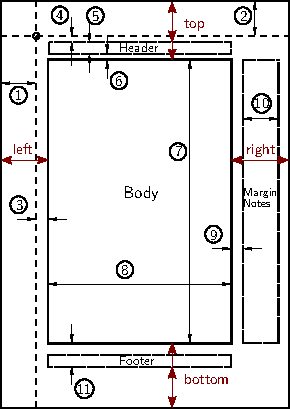
\includegraphics[scale=0.9]{layout.pdf}
\begin{tabular}{rl@{\quad}rl@{\quad}rl}
\ding{192} & 1in + \lstinline+\hoffset+  & \ding{193} & 1in + \lstinline+\voffset+ & \ding{194} & \lstinline+\oddsidemargin+\\
\ding{195} & \lstinline+\topmargin+      & \ding{196} & \lstinline+\headheight+    & \ding{197} & \lstinline+\headsep+\\
\ding{198} & \lstinline+\textheight+     & \ding{199} & \lstinline+\textwidth+     & \ding{200} & \lstinline+\marginparwidth+\\ 
\ding{201} & \lstinline+\marginparwidth+ & \textcircled{\fontsize{1.4mm}{.1mm}\selectfont1\!1} & \lstinline+\footskip+ 
\end{tabular}\\
}
Hint: This image with the current values of the specific document can be
generated by loading the package \texttt{layout} and the command \lstinline+\layout+.
}


% SECTION ====================================================================================
\section{Own Commands and Environments}
% ============================================================================================

\sectionbox{
\subsection{Own Commands in General}
\begin{itemize}
\item 
\lstinline+\newcommand+ doesn't work if the command is already defined: so it's a completely new definition.
\item 
\lstinline+\renewcommand+ works only if the command is already defined: it's a redefinition.
\item 
\lstinline+\providecommand+ works like \lstinline+\newcommand+, but if the command is already defined, the (re)definition is ignored.
\item 
\lstinline+\AtBeginDocument{+\textit{commands}\lstinline+}+ can be helpful.
\end{itemize}
}

\sectionbox{
\subsection[Own Commands]{Own Commands\phantom{g}}\label{owncmds}
\begin{tabular}{@{}ll@{}}
Define:  & \lstinline+\newcommand{\+\textit{cmdname}\lstinline+}{+\textit{commands}\lstinline+}+ \\
Exmp:    & \lstinline+\newcommand{\mytext}{Some text which I need very often.}+\\			
Exmp:    & \lstinline+\newcommand{\diff}{\mathop{}\!\mathrm{\vphantom( d}}+\\			
Params:  & \lstinline+#1+ \dots{} \lstinline+#9+ \\
Define:	& \lstinline+\newcommand[+\textit{paramsquantity}\lstinline+]{\+\textit{cmdname}\lstinline+}{+\textit{cmds} \lstinline+#1+ \dots{}\lstinline+}+\\
Redefine: & \lstinline+\renewcommand[+\textit{paramsquantity}\lstinline+]{\+\textit{cmdname}\lstinline+}{+\textit{commands}\lstinline+}+ \\
Copy:	    & with \texttt{letltxmacro}: \lstinline+\LetLtxMacro{\+\textit{cmdcpyname}\lstinline+}{\+\textit{cmdname}\lstinline+}+ \\[2pt] 
Define:   & \lstinline+\DeclareMathOperator{+\textit{name}\lstinline+}{+\textit{commands}\lstinline+}+\\
Exmp:     & \lstinline+\DeclareMathOperator{\dirac}{\ensuremath{\delta}}+\\
Exmp:     & \lstinline+\DeclareMathOperator{\acrsinh}{arcsinh}+
\end{tabular}%
}

\sectionbox{
\subsection[Own Environments]{Own Environments\phantom{g}}
\begin{tabular}{@{}ll@{}}
Define:  & \lstinline+\newenvironment{+\textit{envname}\lstinline+}{+\textit{cmds begin}\lstinline+}{+\textit{cmds end}\lstinline+}+\\
Params:  & \lstinline+#1+ \dots{} \lstinline+#9+ \\
Define:	& \lstinline+\newenvironment{+\textit{envname}\lstinline+}[+\textit{paramsquantity}\lstinline+]{+\textit{cmds begin} \lstinline+#1+\\
         & \dots{}\lstinline+}{+\textit{cmds end}  \lstinline+#2+ \dots{}\lstinline+}+\\
Exmp:    & \lstinline+\newenvironment{colorpar}[1]{\color{#1}}{\normalcolor}+\\
Use:     & \lstinline+\begin{colorpar}{violet}+ \textit{text} \lstinline+\end{colorpar}+
\end{tabular}%
}

\sectionbox{
\subsection{Some important Variables}
Counters: \lstinline+page+, \lstinline+section+, \lstinline+figure+, \lstinline+equation+;
to get the formatted content of a counter add \lstinline+\the+, e.g. \lstinline+\thepage+\\
Lengths: \lstinline+\textwidth+, \lstinline+\linewidth+, \lstinline+\columnwidth+, \lstinline+\parindent+, \lstinline+\parskip+\\
Change: \lstinline+\setlength+, \lstinline+\addtolength+ 
}

\sectionbox{
\subsection{Helpfull other Commands for defining own Commands}
\begin{itemize}
\item 
\lstinline+\ensuremath+, e.g. \lstinline+$\tx=...$ defines \tx.+
by \lstinline+\newcommand{\tx}{\ensuremath{\tilde{x}}}+
\item Look for \lstinline+\Declare...+ in package documentations.
\item 
Packages: \texttt{etoolbox}, \texttt{xparse}, \texttt{xkeyval}, \texttt{calc}; see also \texttt{tocbasic}.
\end{itemize}
}


% SECTION ====================================================================================
\section{Useful Weblinks and Summary of Packages}
% ============================================================================================
\sectionbox{
\begin{tabular}{p{.31\columnwidth}@{}p{.66\columnwidth}@{}}
Forum          & \url{http://latex.org}\\
Forum (German) & \url{http://golatex.de} \quad \url{http://texwelt.de}\\
FAQ (German)   & \url{https://texfragen.de}\\
PhD Thesis     & \url{https://www.dickimaw-books.com/latex/thesis}\\
\multicolumn{2}{l@{}}{Math \quad~~\url{https://meta.wikimedia.org/wiki/Help:Displaying_a_formula}}\\
Fonts          & \url{http://www.tug.dk/FontCatalogue}\\
Symbols        & \url{https://ctan.org/pkg/comprehensive}\\
Download (Software) & \url{https://tug.org/texlive}\\
CTAN (Packages)     & \url{https://ctan.org}\\
IDEs           & \TeX{}Studio (recommended)\\ 
               & \url{https://texstudio.sourceforge.net} \\ 
               & \TeX{}shop, \TeX{}works, Kile, Lyx, \dots \\	
TU Dresden CD  & \url{https://github.com/tud-cd/tudscr} \\	
Using \LaTeX{} Online & \url{https://de.sharelatex.com}\\
             & \url{https://www.overleaf.com}\\
DANTE e.V.    & \url{https://www.dante.de} 	
\end{tabular}%
}

\sectionbox{
For all packages a documentation can be found with:\\ 
\lstinline+texdoc+ \textit{package name} (or in the Help menu in IDEs)\\
The documentation for \KOMAScript{} can be found with
\lstinline+texdoc scguien+ or \lstinline+texdoc scrguide+ (German)\\
\begin{tabular}{@{}ll@{}}\toprule
\texttt{acro}      &  Acronyms, Glossary\\
\texttt{amsmath,amssymb}   &  Math extended, Math symbols extended \\
\texttt{babel}     &  Language depend issues\\
\texttt{biblatex}  &  Bibliography\\
\texttt{booktabs}  &  Rules in tabular\\
\texttt{csquotes}  &  Quotations esp. in bibliography\\
\texttt{enumitem}  &  Lists extended\\
\texttt{float}     &  Suppress floating, needs \texttt{scrhack} \\
\texttt{fontenc,inputenc}   &  Font encoding, input encoding \\
\texttt{geometry}  &  Page layout, e.g. size\\
\texttt{graphicx}  &  Graphics\\
\texttt{hyperref}  &  Hyperlinks\\
\texttt{listings}  &  Source code listings, needs \texttt{scrhack} sometimes\\
\texttt{longtable} &  Tables longer than a page\\
\texttt{microtype} &  Optical margin alignment\\
\texttt{multicols} &  Multiple columns extended \\
\texttt{pdfpages}  &  Including PDF pages\\
\texttt{scrlayer-scrpage}   &  Page layout, e.g. headings, watermarking \\	
\texttt{setspace}  &  Control line spread, needs \texttt{scrhack} sometimes\\
\texttt{scrhack}   &  Avoid warnings from \texttt{float}, \texttt{listings}, \texttt{setspace}\\
\texttt{subcaption}&  Multiple figures with multiple captions\\
\texttt{textcomp}  &  Text symbols extended\\ 
\texttt{tabularx} | \texttt{tabulary}  &  Tabular extended\\ 
\texttt{upgreek}   &  Upright greek symbols\\
\texttt{wrapfig} | \texttt{floatflt}   & Graphic surrounded by text\\
\texttt{xcolor}    &  Color\\   \bottomrule
\end{tabular}
}


% SECTION ====================================================================================
\section{A Sample Document (output on next page)}\label{sec:inpfile}
% ============================================================================================

\sectionbox{
\lstinputlisting{thesis.tex}
\lstinputlisting{thesis.bib}
}


\includepdfmerge[pages=-, nup=5x2, pagecommand={\thispagestyle{empty}}, frame=true, scale=0.97]{thesis.pdf,1-9,acknowledgements.pdf}
% END \======================================================================
\end{multicols}

% DOCUMENT_END======================================================================
\end{document}